% Régions de confiance jointes à 95 % de (β₁,β₂) quand la corrélation ρ entre les
% deux régresseurs augmente. Avec T^{-1}X'X = [[1,ρ],[ρ,1]], la variance vaut
% σ²/(T(1-ρ²))·[[1,-ρ],[-ρ,1]] : ses vecteurs propres sont (1,-1) et (1,1), de
% valeurs propres σ²/(T(1-ρ)) et σ²/(T(1+ρ)). Les demi-axes de l'ellipse à 95 %
% sont donc sqrt(5,991·σ²/(T(1∓ρ))). Ci-dessous σ²/T = 1 et l'échelle est 0,5.
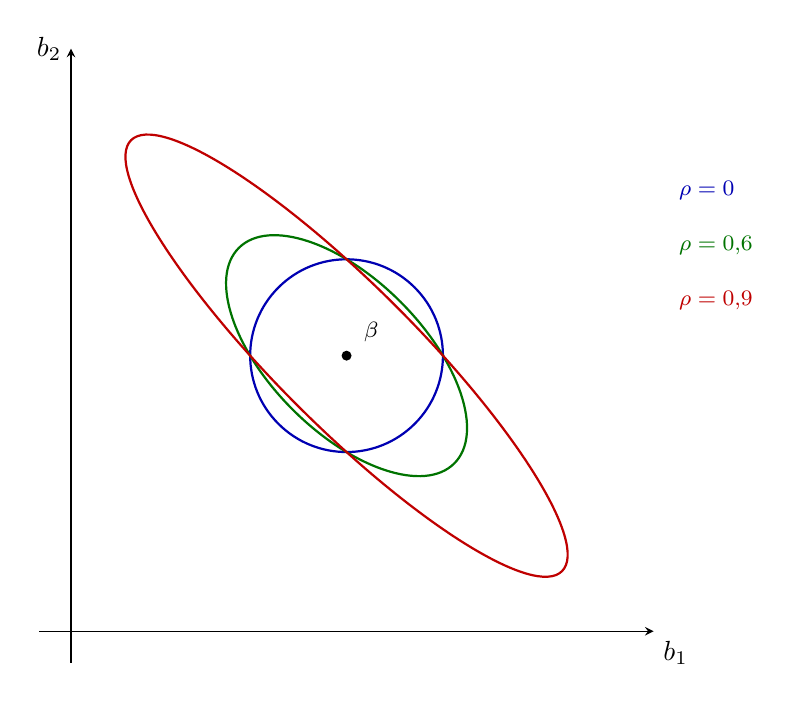
\begin{tikzpicture}[>=stealth]

  \draw[->] (-0.4,0) -- (7.4,0) node[below right] {$b_1$};
  \draw[->] (0,-0.4) -- (0,7.4) node[left] {$b_2$};

  % ρ = 0 : demi-axes 2,448 et 2,448
  \draw[thick, blue!70!black, rotate around={-45:(3.5,3.5)}]
    (3.5,3.5) ellipse [x radius=1.224, y radius=1.224];
  % ρ = 0,6 : demi-axes 3,870 et 1,935
  \draw[thick, green!45!black, rotate around={-45:(3.5,3.5)}]
    (3.5,3.5) ellipse [x radius=1.935, y radius=0.968];
  % ρ = 0,9 : demi-axes 7,740 et 1,776
  \draw[thick, red!75!black, rotate around={-45:(3.5,3.5)}]
    (3.5,3.5) ellipse [x radius=3.870, y radius=0.888];

  \fill (3.5,3.5) circle (1.8pt);
  \node[anchor=south west, font=\footnotesize] at (3.6,3.55) {$\beta$};

  \node[blue!70!black,   anchor=west, font=\footnotesize] at (7.6,5.6) {$\rho = 0$};
  \node[green!45!black,  anchor=west, font=\footnotesize] at (7.6,4.9) {$\rho = 0{,}6$};
  \node[red!75!black,    anchor=west, font=\footnotesize] at (7.6,4.2) {$\rho = 0{,}9$};

\end{tikzpicture}
